
\guideline[g:nontext:figure_same_font]
    {Figures: Use the same font and font sizes as in the running text.}

% bad: different font due to image generating program (or image screenshot, etc.)
\goodbadexample[{\cite[Fig.~6b]{Wetzlinger2021HSCC}}]{
    \begin{center}
        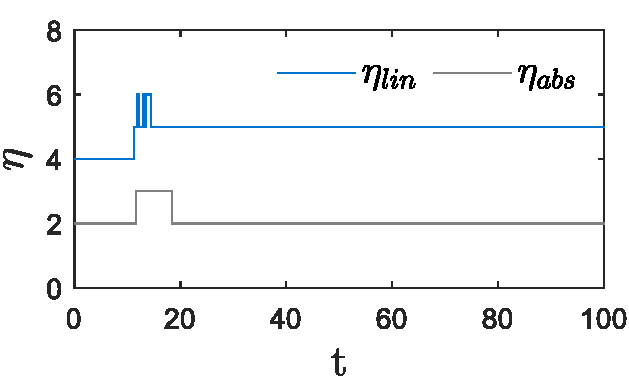
\includegraphics[scale=0.6]{data/figure_same_font_bad.pdf}    
    \end{center}

    Each of the truncation orders $\eta_{\text{lin}}$ and $\eta_{\text{abs}}$ (Fig. 6b) reaches their maximum at the sharp turn as the dynamics there require more terms within the Taylor series of the exponential matrix to provide satisfactory accuracy.
}{
    \begin{center}
        % This file was created by matlab2tikz.
%
%The latest updates can be retrieved from
%  http://www.mathworks.com/matlabcentral/fileexchange/22022-matlab2tikz-matlab2tikz
%where you can also make suggestions and rate matlab2tikz.
%
\definecolor{mycolor1}{rgb}{0.00000,0.36078,0.67059}%
\definecolor{mycolor2}{rgb}{0.89020,0.10588,0.13725}%
%
\tikzsetnextfilename{figure_same_font_good}
\begin{tikzpicture}

\begin{axis}[%
width=5.5cm,
height=2.5cm,
at={(0in,0in)},
scale only axis,
xmin=0.000,
xmax=100.000,
xlabel style={font=\color{white!15!black}},
xlabel={$t$},
ymin=0.000,
ymax=8.000,
ylabel style={font=\color{white!15!black}, yshift=-15pt},
ylabel={$\eta$},
axis background/.style={fill=white},
legend columns = -1,
legend style={legend cell align=left, draw=none, font=\small, align=left, at = {(0.97,0.9)}, anchor=north east},
% legend style={legend cell align=left, font=\small, align=left, draw=white!15!black,
%	at={(-0.1,-0.4)}, anchor=north west,
%	/tikz/column 2/.style={column sep=0.075cm}},
%legend image post style={line width = 1pt},
every tick label/.append style={font=\footnotesize}
]

\addplot [color=mycolor1, line width=0.75pt]
  table[row sep=crcr]{%
0	4 \\
12 4 \\
12.5 4 \\
12.5 5 \\
13 5 \\
13 6 \\
13.5 6 \\
13.5 5 \\
14.5 5 \\
14.5 6 \\
14.6 6 \\
14.6 5 \\
14.7 5 \\
14.7 6 \\
14.8 6 \\
14.8 5 \\
14.9 5 \\
14.9 6 \\
15.0 6 \\
15.0 5 \\
15.1 5 \\
15.1 6 \\
16 6 \\
16 5 \\
100 5 \\
};
\addlegendentry{$\eta_{\text{lin}}$}

\addplot [color=gray, line width=0.75pt]
  table[row sep=crcr]{%
0 2 \\
13 2 \\
13 3 \\
19 3 \\
19 2\\
100	2\\
};
\addlegendentry{$\eta_{\text{abs}}$}

\end{axis}

\end{tikzpicture}%
    \end{center}

    Each of the truncation orders $\eta_{\text{lin}}$ and $\eta_{\text{abs}}$ (Fig. 6b) reaches their maximum at the sharp turn as the dynamics there require more terms within the Taylor series of the exponential matrix to provide satisfactory accuracy.
}

\noindent Using the same font and font sizes in figures as in the running text allows the figure to blend seamlessly with the rest of the document, contributing to a cohesive overall appearance.
This is most easily achieved with the \LaTeX{} package \emph{TikZ}, as it compiles the text in figures using the same settings as the rest of the document.
